
\usepackage[spanish]{babel}
\usepackage[ansinew]{inputenc}
\usepackage{amsmath}
\usepackage{enumerate}
\usepackage{latexsym}
\usepackage[noend]{algorithmic}
\usepackage{algorithm}

\title{Estructuras de Datos\\ Conjunto y Diccionario}
\author{Algoritmos y Estructuras de Datos \\
Programaci�n Estructurada}
\date{}

\newcommand{\pseudohrule}{\vskip 5pt \hrule}

\newenvironment{pseudo}[1][\normalsize]{
\begin{figure}
#1
\begin{semiverbatim}
}{
\end{semiverbatim}
\normalsize
\end{figure}
}

\setlength{\parskip}{3pt plus 1pt minus 1pt}

\begin{document}

\begin{frame}
\titlepage
\end{frame}

%%%%%%%%%%%%%%%%%%%%%%%%%%

\begin{frame}[fragile]{Repaso}

\uncover<1->{
\begin{block}{Especificaci�n}
La especificaci�n de un algoritmo es un contrato entre el programador y el usuario en donde se definen 
cuales son los datos de entrada, la precondici�n y la postcondici�n del mismo.
\end{block}
}

\uncover<2->{
\begin{block}{Correctitud}
Un algoritmo es correcto cuando siempre que vale la precondici�n podemos asegurar que el programa termina y la postcondici�n se cumple.
\end{block}
}

\end{frame}

%%%%%%%%%%%%%%%%%%%%%%%%%%

\begin{frame}[fragile]{Estructuras de datos}

La clase pasada vimos \textbf{lista} como una nueva estructura de datos que nos permite guardar elementos de manera ordenada. 

Es importante saber cu�ndo nos conviene usar cada estructura:
\begin{itemize}
\item el arreglo permite acceso inmediato a cada elemento, siendo m�s eficiente cuando tenemos una cantidad fija de elementos
\item la lista permite insertar y eliminar elementos f�cilmente, siendo ideal para cuando no sabemos cu�ntos elementos tenemos que manejar
\end{itemize}

\uncover<2>{
Hoy veremos otras dos estructuras de datos: \textbf{conjunto} y \textbf{diccionario}.
}

\end{frame}

%%%%%%%%%%%%%%%%%%%%%%%%%%

\begin{frame}[fragile]{Conjunto}

El \textbf{conjunto} es una estructura de datos que nos permite guardar elementos \textbf{sin repetir} y \textbf{sin un orden en particular}.

\begin{center}
\begin{figure}
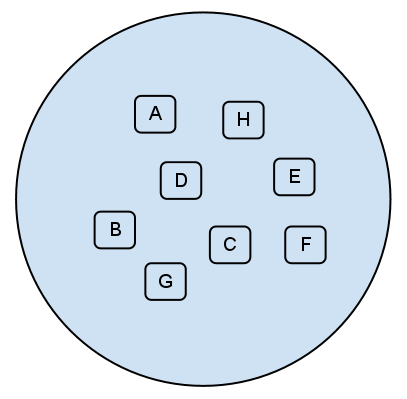
\includegraphics[scale=0.4]{C08/STLSet.png}
\end{figure}
\end{center}

\end{frame}

%%%%%%%%%%%%%%%%%%%%%%%%%%

\begin{frame}[fragile]{Agregar un elemento}

Al agregar un nuevo elemento al conjunto, no indicamos la posici�n, pues no hay un orden en el cual se guarden los elementos. Notemos que si el elemento ya exist�a, no se lo agrega nuevamente.

\begin{center}
\begin{figure}
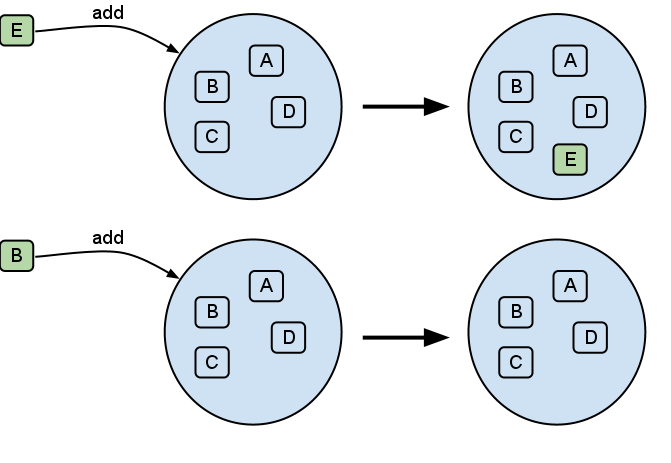
\includegraphics[scale=0.35]{C08/STLSetAdd.png}
\end{figure}
\end{center}

Al iterar los elementos del conjunto, estos pueden aparecer en cualquier orden, no necesariamente en el de inserci�n.

\end{frame}

%%%%%%%%%%%%%%%%%%%%%%%%%%

\begin{frame}[fragile]{Operaciones de Conjunto}

\begin{itemize}
\item \texttt{iterar}\\permite iterar sobre los elementos del conjunto usando una estructura \textit{para cada}
\item \texttt{int tama�o()}\\cantidad de elementos del conjunto
\item \texttt{bool agregar(elem)}\\agrega el elemento \textit{elem} al conjunto si no exist�a, caso en el que devuelve \textit{true}, \textit{false} si no
\item \texttt{void eliminar(elem)}\\elimina el elemento \textit{elem} del conjunto si exist�a
\item \texttt{bool contiene(elem)}\\indica si el conjunto contiene al elemento \textit{elem}
\end{itemize}

\end{frame}

%%%%%%%%%%%%%%%%%%%%%%%%%%

\begin{frame}[fragile]{Ejemplo de uso}

\begin{pseudo}[\small]
conjunto(string) c

c.agregar('juan')     -> true
c.agregar('pedro')    -> true
c.agregar('carlos')   -> true
c.tama�o()            -> 3

c.agregar('juan')     -> false
c.tama�o()            -> 3

c.eliminar('juan')
c.tama�o()            -> 2

para cada string nombre en c
  imprimir nombre
-> 'carlos', 'pedro' 
\end{pseudo}

\end{frame}

%%%%%%%%%%%%%%%%%%%%%%%%%%

\begin{frame}[fragile]{Diccionario}

As� como antes ten�amos estructuras de datos que guardaban un \textbf{tipo} de elementos...
\begin{itemize}
\item arreglo de booleanos
\item lista de enteros
\item conjunto de strings
\end{itemize}

El tipo de datos \textbf{diccionario} o \textbf{mapa} nos permite guardar una asociaci�n entre elementos de dos tipos diferentes, teniendo as� por ejemplo un...
\begin{itemize}
\item diccionario de strings en enteros
\end{itemize}

\end{frame}

%%%%%%%%%%%%%%%%%%%%%%%%%%

\begin{frame}[fragile]{Diccionario}

El diccionario puede verse como un conjunto de \textbf{claves}, cada una con un \textbf{valor} asociado, no necesariamente del mismo tipo. 

Un diccionario puede guardar, por ejemplo, para cada \textit{alumno} de un curso, su \textit{nota} en un examen:

\begin{pseudo}[\small]
diccionario de string en int
\pseudohrule
'Juan G�mez': 7
'Carlos Fern�ndez': 4
'Guillermo Mart�nez': 9
'Fernando Gonz�lez': 7
\end{pseudo}

Los diccionarios, de forma similar al conjunto, \textbf{no admiten claves repetidas} (s� valores repetidos), y \textbf{no se guardan en ning�n orden en particular}.

\end{frame}

%%%%%%%%%%%%%%%%%%%%%%%%%%

\begin{frame}[fragile]{Operaciones de Diccionario}

\begin{itemize}
\item \texttt{iterador claves()}\\permite iterar sobre las \textbf{claves} del diccionario usando una estructura \textit{para cada}
\item \texttt{int tama�o()}\\cantidad de elementos del diccionario
\item \texttt{[clave]}\\devuelve el \textit{valor} asignado a la \textit{clave}
\item \texttt{[clave]=valor}\\asigna a la \textit{clave} indicada el nuevo \textit{valor}, agregando la clave al diccionario si no exist�a
\item \texttt{void eliminar(clave)}\\elimina la \textit{clave} del diccionario si exist�a
\item \texttt{bool contiene(clave)}\\indica si el diccionario contiene la clave indicada
\end{itemize}

\end{frame}

%%%%%%%%%%%%%%%%%%%%%%%%%%

\begin{frame}[fragile]{Resumiendo}

Vimos dos nuevas estructuras de datos, que no guardan los elementos en ning�n orden en particular:

\begin{block}{Conjunto}
Guarda elementos sin repetir y permite f�cilmente agregar, eliminar y chequear pertenencia, as� como recorrer los elementos que contiene.
\end{block}

\begin{block}{Diccionario}
Guarda pares de \textit{clave}-\textit{valor}, siendo las claves �nicas, permitiendo f�cilmente asignar nuevos valores a las claves y obtener el conjunto de claves.
\end{block}

\end{frame}

%%%%%%%%%%%%%%%%%%%%%%%%%%

\begin{frame}[fragile]{En conclusi�n...}

Tenemos las siguientes estructuras de datos para guardar elementos:

\begin{itemize}
\item Arreglo
\item Lista
\item Conjunto
\item Diccionario
\end{itemize}

Es importante saber cu�ndo nos conviene usar cada una dependiendo del problema que estemos resolviendo y de qu� tengamos que modelar.

\end{frame}

\end{document}

